% !TeX spellcheck = en_US
\chapter{Deep Learning for CV}
\todo{}

\section{Image-to-Image Translation}
Image-to-image translation is a class of computer vision problems where the goal is to learn the mapping between an input image and an output image. Recent approaches utilize \ac{GAN}. It has various applications \cite{isola2017image, zhu2017unpaired}, \eg:
\begin{itemize}
	\item Domain adaptation
	\item Semantic label $\leftrightarrow$ photo
	\item Map $\leftrightarrow$ aerial photo
	\item Edges $\rightarrow$ photo
	\item BW $\rightarrow$ color photos
	\item Day $\rightarrow$ night
	\item Photo with missing pixels $\rightarrow$ inpainted photo (recovering)
\end{itemize}

\subsection{pix2pix}
\texttt{pix2pix} uses \ac{CGAN} idea with U-Net architecture \cite{isola2017image}.
\begin{figure}[hbt!]
	\centering
	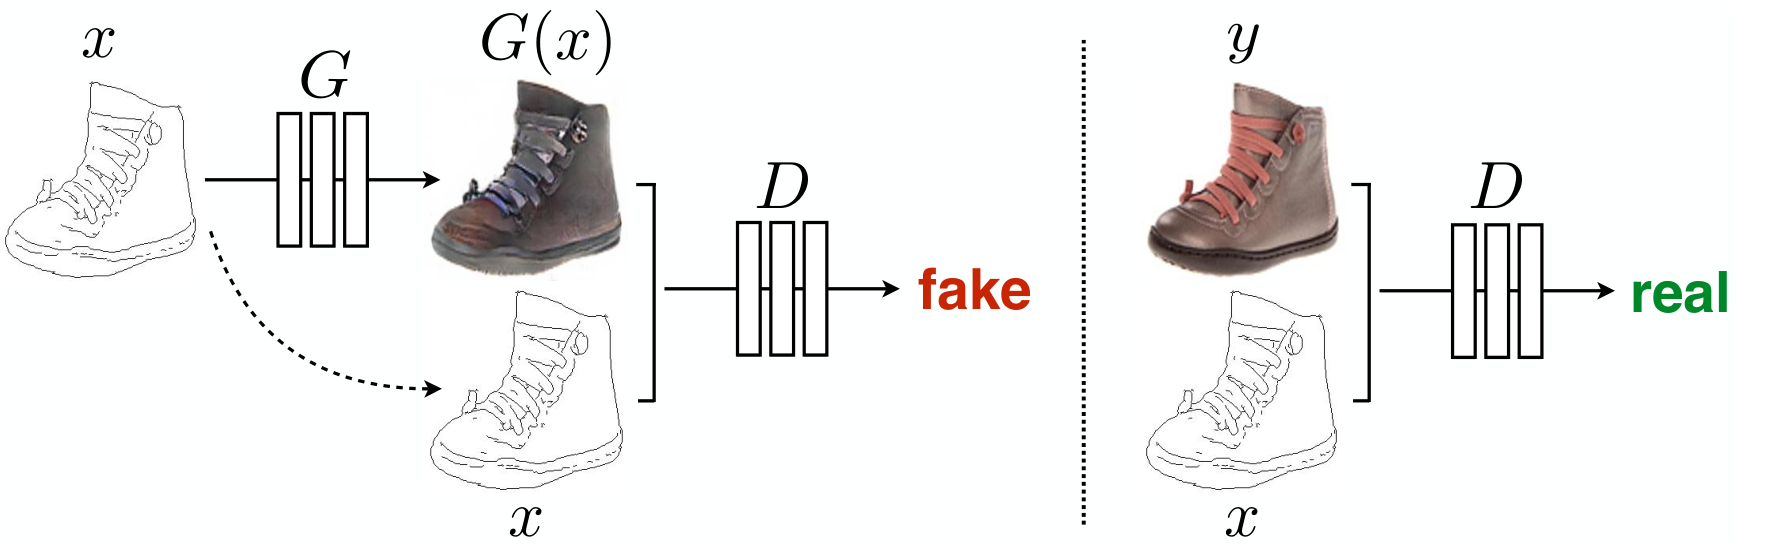
\includegraphics[width=0.9\textwidth]{pix2pix.png}
	\caption{Training a \ac{CGAN} to map edges $\rightarrow$ photo. Both the discriminator and generator are conditioned on the input $x$. \cite{isola2017image}}
\end{figure}

The loss function of \texttt{pix2pix} combines \ac{CGAN} objective with L1 distance with ground-truth images. L1 distance is prefer over L2 because L1 encourages less blurring effect.
\begin{align}
	\mathcal{L}_{GAN}(G,D) &= \mathbb{E}_y [\log D(y)] + \mathbb{E}_z [\log (1-D(G(z)))]\\
	\mathcal{L}_{CGAN}(G,D) &= \mathbb{E}_{x,y} [\log D(x,y)] + \mathbb{E}_{x,z} [\log (1-D(x,G(x,z)))]\\
	\mathcal{L}_{L1}(G) &= \mathbb{E}_{x,y,z} \big[ ||y-G(x,z)||_1 \big]\\
	G* &= \arg \underset{G}{\min} \underset{D}{\max} \mathcal{L}_{CGAN}(G,D) + \lambda \mathcal{L}_{L1}(G)
\end{align}

\note In implementation, the noise $z$ is accounted as DropOut percentage.

\subsection{CycleGAN}
Cycle\ac{GAN} addresses the problem when there is no \hlb{available paired training data}. By considering cycle consistency losses, it limits the mapping functions. \cite{zhu2017unpaired}
\begin{align}
	&G: X \rightarrow Y &&-\text{mapping from domain $X$ to domain $Y$}\\
	&F: Y \rightarrow X &&-\text{mapping from domain $Y$ to domain $X$}\\
	&F(G(x)) \approx x &&-\text{forward cycle consistency}\\
	&G(F(y)) \approx y &&-\text{backward cycle consistency}
\end{align}
\begin{align}
	\mathcal{L}_{GAN_1} (G, D_Y, X, Y) &= \mathbb{E}_{y \sim p_{data}(y)}[\log D_Y(y)] + \mathbb{E}_{x \sim p_{data}(x)} [\log (1 - D_Y(G(x)))]\\
	\mathcal{L}_{GAN_2} (F, D_X, X, Y) &= \mathbb{E}_{x \sim p_{data}(x)}[\log D_X(x)] + \mathbb{E}_{y \sim p_{data}(y)} [\log (1 - D_X(F(y)))]\\
	\mathcal{L}_{cyc}(G,F) &= \mathbb{E}_{x \sim p_{data}(x)}\big[||F(G(x))-x||_1 \big] + \mathbb{E}_{y \sim p_{data}(y)} \big[||G(F(y))-y||_1\big]\\
	\mathcal{L}(G, F, D_X, D_Y) &= \mathcal{L}_{GAN_1} (G, D_Y, X, Y) + \mathcal{L}_{GAN_2} (F, D_X, X, Y) + \lambda \mathcal{L}_{cyc}(G,F)\\
	G^*, F^* &= \arg\underset{G, F}{\min}\underset{D_X, D_Y}{\max} \mathcal{L}(G, F, D_X, D_Y)
\end{align}
\begin{figure}[hbt!]
	\centering
	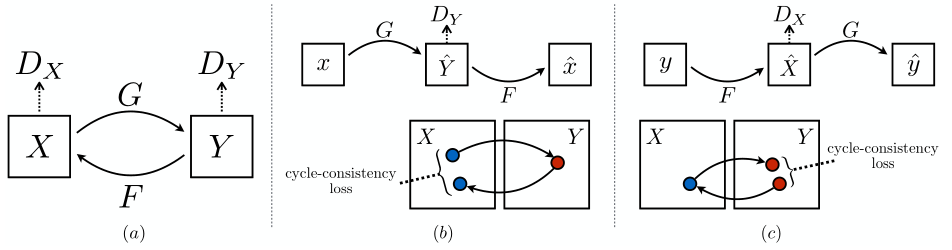
\includegraphics[width=\textwidth]{cyclegan.png}
	\caption{Cycle\ac{GAN} structure with 4 networks. \cite{zhu2017unpaired}}
\end{figure}

\note
\begin{itemize}
	\item The authors mention that experiment the cycle consistency loss as adversarial loss leads to no improved performance.
	\item Cycle\ac{GAN}'s results are not significantly better than pix2pix's.
	\item Perform well on tasks relating color transformation (\eg style transfer: picture $\leftrightarrow$ paintings, horse $\leftrightarrow$ zebra, winter $\leftrightarrow$ summer), but not so good with \hlb{geometric changes} (dog $\leftrightarrow$ cat).
\end{itemize}

\section{Neural Style Transfer}
Style transfer is similar to image-to-image translation, but doesn't require a dataset from each style. It instead runs an iterative optimization procedure on two given images.

\subsection{Artistic Style Transfer}
The first work is by \citeaus{gatys2015neural}. The authors manage to separate image content and image style. Given a \ac{CNN}, at the $l^{th}$ layer, there is $N_l$ distinct filters, thus, leads to $N_l$ feature maps of size $M_l$.
\begin{itemize}
	\item The image content is represented in matrix $F^l \in \mathcal{R}^{N_l \times M_l}$, which is the concatenation of these feature maps. $F^l_{ij}$ is the activation of the $i^{th}$ filter at position $j$ in $l^{th}$ layer. The authors prove this by trying to reconstruct the image from these feature maps.
	\begin{align}
		&\vec{p} &&-\text{original image}\\
		&\vec{x} &&-\text{generated image}\\
		&F^l_{ij} &&-\text{the original image's content }\\
		&P^l_{ij} &&-\text{the generated image's content}\\
		&\mathcal{L}_{content}(\vec{p}, \vec{x}, l) = \frac{1}{2} \sum_{i,j} \left( F^l_{ij} - P^l_{ij} \right) ^2 &&-\text{the content loss}
	\end{align}
	\item The image style is represented in the Gram matrix $G^l \in \mathcal{R}^{N_l \times N_l}$, where $G_{ij}^l$ is the correlation between feature map in the $l^{th}$ layer:
	\begin{equation}
		G_{ij}^l = \sum_k F_{ik}^l F_{jk}^l
	\end{equation}
	\begin{align}
		&\vec{a} &&-\text{artwork}\\
		&\vec{x} &&-\text{generated image}\\
		&A^l &&-\text{the artwork's style representation}\\
		&G^l &&-\text{the generated image's style representation}\\
		&E_l = \frac{1}{4 N^2_l M^2_l} \sum_{i,j} \left( G_{ij}^l - A_{ij}^l \right)^2 &&-\text{style representation loss at $l^{th}$ layer}	\\
		&\mathcal{L}_{style}(\vec{a}, \vec{x}) = \sum_{l=0}^L w_l E_l &&-\text{the style loss}
	\end{align}
\end{itemize}
\begin{align}
	&\mathcal{L}_{total}(\vec{p}, \vec{a}, \vec{x}) =  \alpha \mathcal{L}_{content}(\vec{p}, \vec{x})+ \beta \mathcal{L}_{style}(\vec{a}, \vec{x}) &&-\text{total loss}
\end{align}

The algorithm applies gradient descent to minimize the above loss with $\vec{x}$ as a white noise image in the beginning.

\subsection{Artistic Style Transfer for Videos}
Applying the above approach to video leads to terribly inconsistent results. \citeaus{ruder2016artistic} improve by adding additional improvements:
\begin{itemize}
	\item Short-term consistency by initialization: Estimate the optical flow between image $p^{(i)}$ and $p^{(i+1)}$. The generated image $x^{(i+1)}$ will not be initialized with a white noise image, but a warped image from the previous one: $x'^{(i+1)} = \omega_i^{i+1} (x^{(i)})$. Here $\omega_i^{i+1}$ denotes the warping function using the estimated optical flow.
	\item Temporal consistency loss
	\item Long-term consistency
	\item Multi-pass algorithm
\end{itemize}

\subsection{Fast Artistic Style Transfer}
The above approaches for style transfer require an iterative optimization process for each image. \citeaus{johnson2016perceptual} propose a training pipeline to simplify this procedure. By learning a network that minimize the same loss, the output now requires only one single run. It does loss some of the temporal consistency when applying to videos, but it's running in real-time.
\begin{figure}[hbt!]
	\centering
	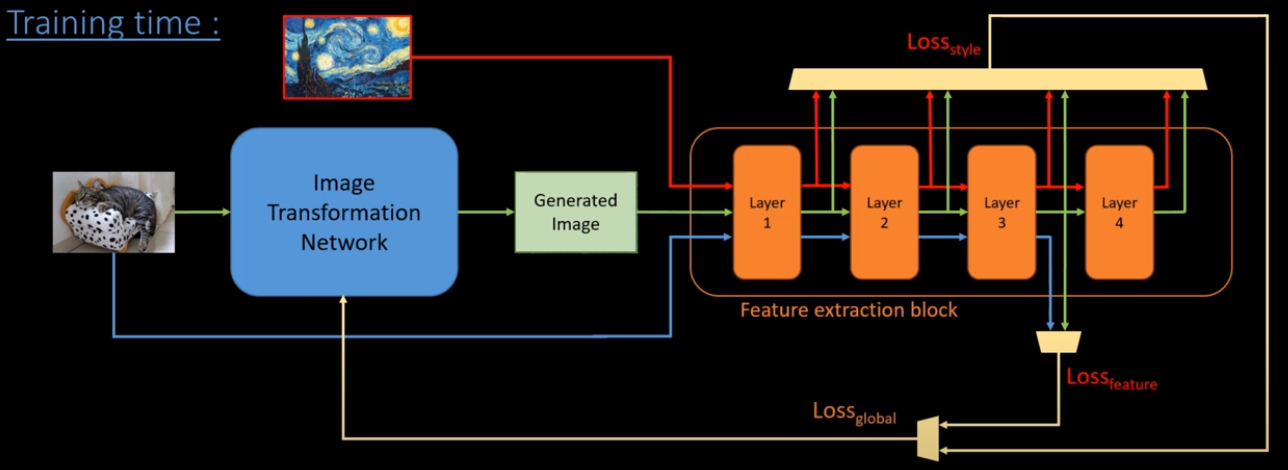
\includegraphics[width=\textwidth]{fast-artistic-style-transfer.png}
	\caption{Training pipeline (\href{https://youtu.be/VQEMptfWpLk}{src}) \cite{johnson2016perceptual}}
\end{figure}

\section{Super Resolution}
\href{https://youtu.be/KULkSwLk62I}{Youtube: How Super Resolution Works}
\begin{itemize}
	\item Use \ac{SSIM} \cite{wang2009mean, wang2004image}
\end{itemize}
\subsection{SRCNN}
\begin{figure}[hbt!]
	\centering
	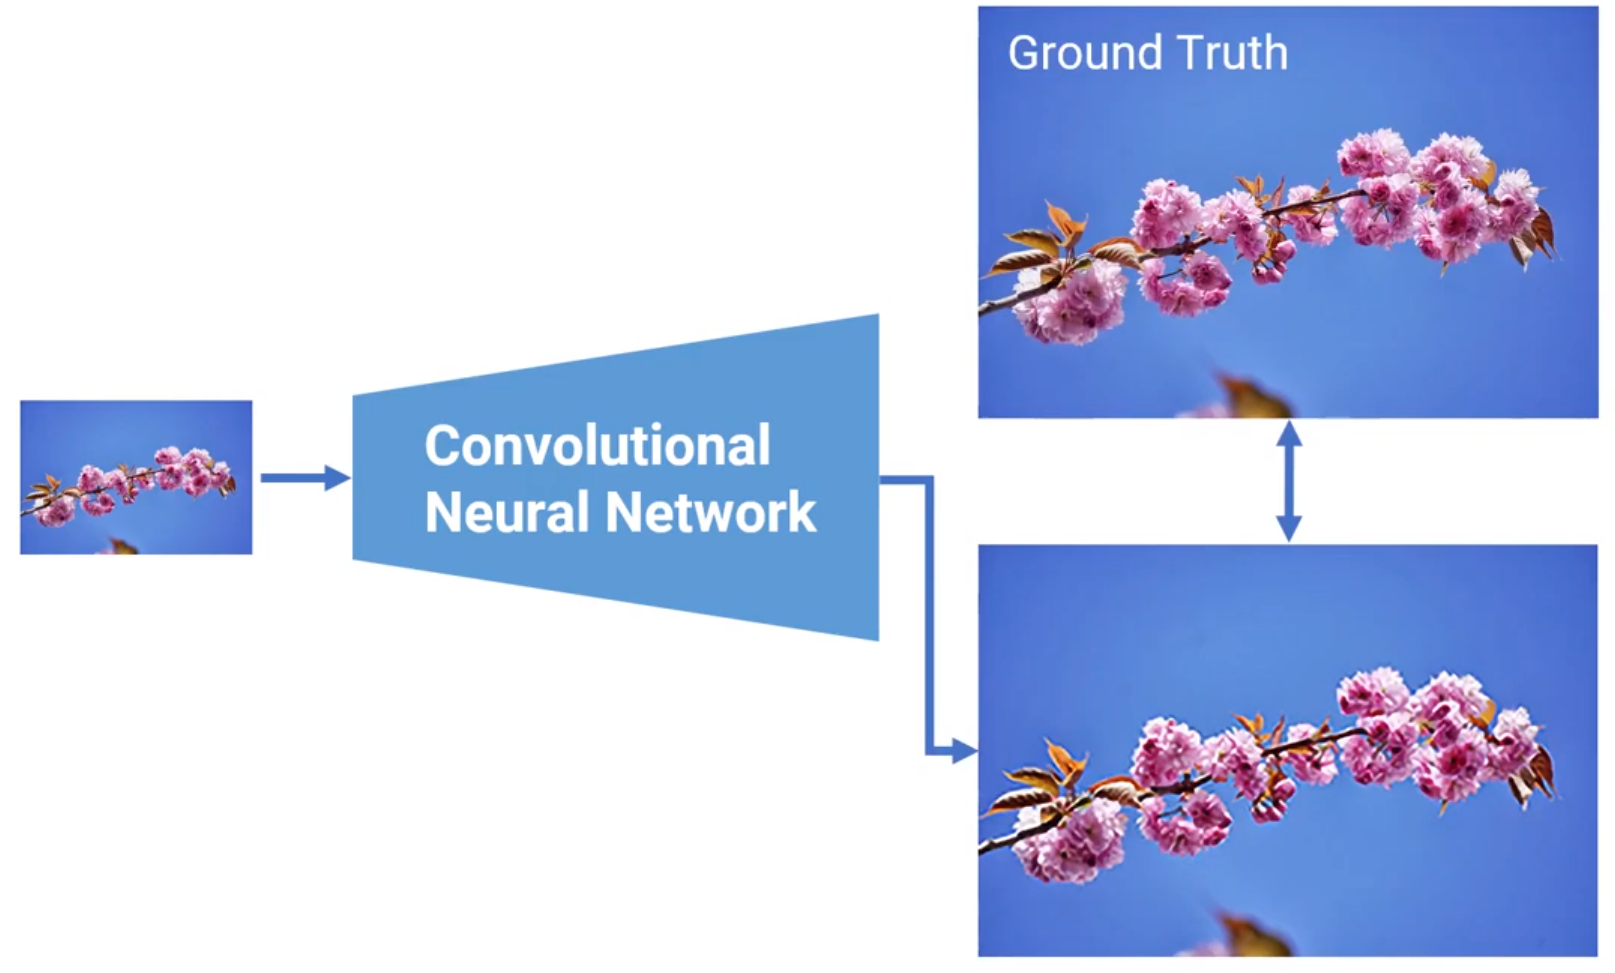
\includegraphics[width=0.7\textwidth]{SRCNN.png}
	\caption{\ac{SRCNN} training \cite{dong2015image}}
\end{figure}

\subsection{SRGAN}
\begin{figure}[hbt!]
	\centering
	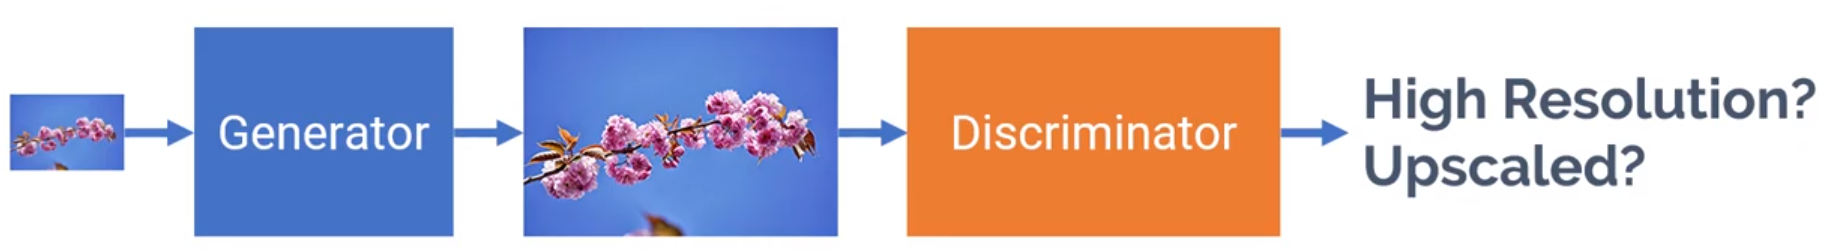
\includegraphics[width=\textwidth]{SRGAN.png}
	\caption{\ac{SRGAN} training \cite{ledig2017photo}}
\end{figure}

\subsection{ESRGAN}
\ac{ESRGAN} \cite{wang2018esrgan}
\begin{itemize}
	\item Remove Batch Normalization
	\item More layers and connections: residual scaling
	\item Modify the VGG loss
	\item Relativistic discriminator
\end{itemize}

\section{Code Examples}
\begin{itemize}
	\item \href{https://www.tensorflow.org/tutorials/generative/pix2pix}{\texttt{Tensorflow}'s tutorial: pix2pix}
	\item \href{https://www.tensorflow.org/tutorials/generative/cyclegan}{\texttt{Tensorflow}'s tutorial: CycleGAN}
	\item \href{https://github.com/manuelruder/artistic-videos}{\texttt{Github} source code: Artistic Style Transfer for Videos}
	\item \href{https://www.tensorflow.org/tutorials/generative/style_transfer}{\texttt{Tensorflow}'s tutorial: Neural style transfer}
	\item \href{https://www.tensorflow.org/hub/tutorials/tf2_arbitrary_image_stylization}{\texttt{Tensorflow}'s tutorial: Fast Style Transfer}
\end{itemize}
